\documentclass[a4paper,12pt]{report}
\usepackage{graphicx}
\usepackage{hyperref}
\usepackage[T1]{fontenc}
\usepackage[utf8]{inputenc}
\usepackage[english,italian]{babel}
\usepackage{setspace}
\usepackage[paper=a4paper,margin=1in]{geometry}
\usepackage{lipsum}
\usepackage{microtype}
\usepackage{times}
\usepackage{xcolor}
\usepackage{hyperref}
\graphicspath{ {images/} }

\title{Test Document}
\author{Simone Renzo}
\date{Febbraio 2021}

%%%%********************************************************************
% fancy quotes
\definecolor{quotemark}{gray}{0.7}
\makeatletter
\def\fquote{%
	\@ifnextchar[{\fquote@i}{\fquote@i[]}%]
}%
\def\fquote@i[#1]{%
	\def\tempa{#1}%
	\@ifnextchar[{\fquote@ii}{\fquote@ii[]}%]
}%
\def\fquote@ii[#1]{%
	\def\tempb{#1}%
	\@ifnextchar[{\fquote@iii}{\fquote@iii[]}%]
}%
\def\fquote@iii[#1]{%
	\def\tempc{#1}%
	\vspace{1em}%
	\noindent%
	\begin{list}{}{%
			\setlength{\leftmargin}{0.1\textwidth}%
			\setlength{\rightmargin}{0.1\textwidth}%
		}%
		\item[]%
		\begin{picture}(0,0)%
			\put(-15,-5){\makebox(0,0){\scalebox{3}{\textcolor{quotemark}{``}}}}%
		\end{picture}%
		\begingroup\itshape}%
	%%%%********************************************************************
	\def\endfquote{%
		\endgroup\par%
		\makebox[0pt][l]{%
			\hspace{0.8\textwidth}%
			\begin{picture}(0,0)(0,0)%
				\put(15,15){\makebox(0,0){%
						\scalebox{3}{\color{quotemark}''}}}%
		\end{picture}}%
		\ifx\tempa\empty%
		\else%
		\ifx\tempc\empty%
		\hfill\rule{100pt}{0.5pt}\\\mbox{}\hfill\tempa,\ \emph{\tempb}%
		\else%
		\hfill\rule{100pt}{0.5pt}\\\mbox{}\hfill\tempa,\ \emph{\tempb},\ \tempc%
		\fi\fi\par%
		\vspace{0.5em}%
	\end{list}%
}%
\makeatother
%%%%********************************************************************

\begin{document}
	
	\begin{titlepage}
		\noindent
		\begin{minipage}[t]{0.19\textwidth}
			\vspace{-4mm}{
\includegraphics[scale=1.15]{logo_unimib.pdf}}
		\end{minipage}
		\begin{minipage}[t]{0.81\textwidth}
			{
				\setstretch{1.42}
				{\textsc{Università degli Studi di Milano - Bicocca}} \\
				\textbf{Scuola di Scienze} \\
				\textbf{Dipartimento di Informatica, Sistemistica e Comunicazione} \\
				\textbf{Corso di laurea in Informatica} \\
				\par
			}
		\end{minipage}
		
		\vspace{40mm}
		
		\begin{center}
			{\LARGE{
					\setstretch{1.2}
					\textbf{DevOps: studio e implementazione \\ di una pipeline di CI e CD \\ nel progetto Sphere}
					\par
			}}
		\end{center}
		
		\vspace{40mm}
		
		\noindent
		{\large \textbf{Relatore:} Prof. Mariani Leonardo} \\
		
		\noindent
		{\large \textbf{Tutor Aziendale:} Dott. Mesiano Cristian}
		
		\vspace{15mm}
		
		\begin{flushright}
			{\large \textbf{Relazione della prova finale di:}} \\
			\large{Renzo Simone} \\
			\large{Matricola 781616} 
		\end{flushright}
		
		\vspace{40mm}
		\begin{center}
			{\large{\bf Anno Accademico 2020-2021}}
		\end{center}
		
		\restoregeometry
		
	\end{titlepage}
	
	\selectlanguage{english}
	\begin{abstract}
		In un mondo in continuo sviluppo, la necessità di adattarsi velocemente al cambiamento è spesso
		ciò che permette di contraddistinguere realtà di successo dalle fallimentari.
		Il software è probabilmente uno dei prodotti che più segue questa filosofia di cambiamento repentino,
		con la continua uscita di nuove tecnologie, nuove metodiche e la conseguente necessità di cambiare spesso
		rotta e requisiti in base alle necessità o al mercato di riferimento.
		
		La nascita di metodi \emph{Agile} e di nuove filosofie improntate all'unire ciò che prima era separato,
		in un unico processo, hanno permesso di adattarsi con successo ai cambiamenti, rendendo l'industria del
		software quella più all'avanguardia e resiliente nel tempo, continuando tutt'oggi a migliorarsi sempre più.
		
 		\begin{fquote}[Charles Darwin]
		 	It is not the strongest of the species that survives, nor the most intelligent that survives.
		 	It is the one that is the most adaptable to change.
	 	\end{fquote}
	\end{abstract}

	\selectlanguage{italian}
	\tableofcontents
	
	\chapter{Introduzione}
	
	\section{Il Contesto Aziendale}
	
		\subsection{Storia}
		
			\lipsum[1]
		
		\subsection{Il progetto Sphere}
		
			\lipsum[2]
	
		\subsection{Profilo personale in azienda}
		
			In PerceptoLab Srl, il candidato è stato assunto in Giugno 2020, con ruolo di Infrastructure \& DevOps Engineer,
			integrato nel team di Backend Development.
	
	\section{Scopo del Project Work}
	
		\subsection{Obiettivi}
	
			Il Project Work ha come scopo il design e l'implementazione di un processo che includa una Pipeline di Continuous
			Integration e di Continuous Delivery, nell'ambito del progetto Sphere.
			
			In particolare si prefigge questi obiettivi:
			\begin{enumerate}
				\item Creazione di un processo di \emph{Continuous Integration} per il repository progettuale, mediante l'uso di tool per il testing automatico e per la gestione delle Pull Request, con integrazione per build in ambiente macOS;
				\item Creazione di un processo di \emph{Continuous Delivery} per la creazione di immagini Docker mediante utilizzo di tag specifici su repository e delivery degli artefatti su registry remoto;
				\item Integrazione nella pipeline DevOps di \emph{analisi statica e dinamica} del codice mediante tools dedicati e definizione di quality gates in base alle necessità progettuali;
				\item Creazione e gestione dell'infrastruttura (basata su \emph{Amazon Web Services}) necessaria al deployment dei servizi sviluppati nel progetto aziendale.
			\end{enumerate}
	
		\subsection{Pianificazione del Lavoro}
	
			Il Project Work si è svolto durante il periodo di 3 mesi tra l'1 Ottobre 2020 ed il 31 Dicembre 2020, in modalità di remote
			working con l'utilizzo di tools di collaboration integrati in Google GSuite (Google Chat, Meets) e nella suite Atlassian
			(Bitbucket, Jira, Confluence).
			
			INSERIRE UN GANTT.
	
		\subsection{Prodotti Finali}
		
			I prodotti del project work saranno i seguenti:
			\begin{itemize}
				\item Analisi dei Requisiti per i processi da implementare
				\item Pipeline di Continuous Integration per i servizi di Backend e Mobile
				\item Pipeline di Continuous Delivery per i servizi di Backend (Docker Containers)
				\item Quality Assurance Gates basati sulla analisi dei test e del codice con tools dedicati
				\item Infrastruttura basata su Amazon Web Services (Risorse Cloud, VMs) per gestire i processi descritti.
			\end{itemize}
	
	\chapter{Modelli di Sviluppo del Software}
	
		\section{Il ciclo di vita del software}
	
			\begin{figure}[h]
				\centering
				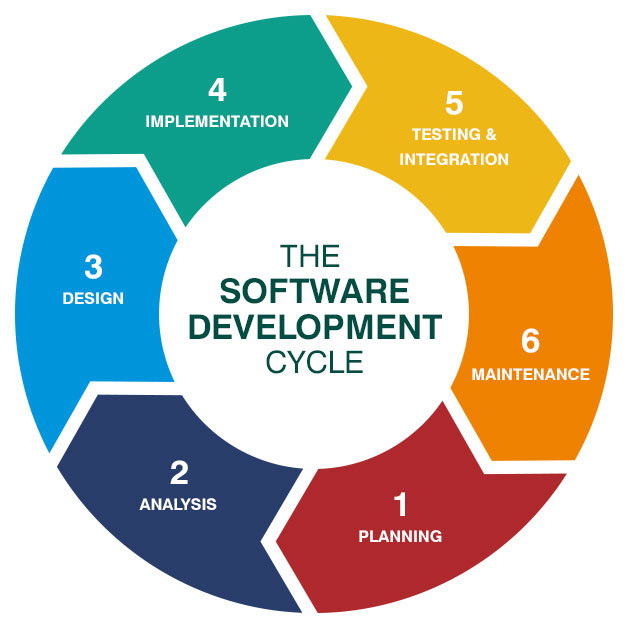
\includegraphics[width=0.4\textwidth]{sdlc}
				\caption{Software Development Lifecycle}
				\label{fig:sdlc}
			\end{figure}
	
			\subsection{Le fasi del ciclo di vita}
	
				Il ciclo di vita del software si riferisce ad una metodologia che permetta di ottenere software di massima qualità
				al minimo costo di produzione e nel minor tempo possibile, dividendo la sua vita in diverse fasi consequenziali:
				\begin{enumerate}
					\item Planning e Analisi
					\item Design
					\item Implementazione
					\item Testing e Integrazione
					\item Manutenzione
				\end{enumerate}
				
				\paragraph{Planning e Analisi}
				Si analizzano i sistemi esistenti per i cambiamenti necessari ed il problema da risolvere in termini di software development.
				Questa fase crea in output una serie di \emph{Requisiti} che possono essere Funzionali, Non Funzionali, o di Dominio, ed un piano
				di lavoro per sviluppare tali requisiti in un tempo definito (ma, come vedremo, variabile in metodi \emph{Agile}).
				Le definizioni di tali requisiti sono dettate dallo standard \href{https://standards.ieee.org/standard/610_12-1990.html}{\emph{IEEE 610.12-1990}}.
				
				\paragraph{Design}
				I requisiti vengono trasformati in una \emph{specifica di Design} (architetturale ed implementativa), che verrà in seguito analizzata
				dagli \emph{stakeholders}, ottenendo così feedback e suggerimenti in base alle esigenze. In questa fase diventa cruciale implementare
				un sistema per incorporare i feedback così da migliorare il design finale ed evitare costi aggiuntivi a fine sviluppo.
				
				\paragraph{Implementazione}
				Questa fase inizia lo sviluppo del software in se, seguendo la specifica di design della fase precedente, ed utilizzando convenzioni,
				code style, pratiche e linee guida comuni per tutti i soggetti coinvolti nello sviluppo. L'utilizzo di linee guida comuni permette di
				evitare fraintendimenti all'interno del team di sviluppo, e di facilitare le fasi future di manutenzione.
				
				\paragraph{Testing e Integrazione}
				Il software sviluppato viene sottoposto a test per difetti e mancanze, risolvendo i problemi trovati lungo il percorso e migliorando
				le feature implementate fino ad arrivare ad una qualità in linea con le specifiche originali.
				In seguito, viene integrato con il resto dell'ambiente mediante deployment, così da poterlo iniziare ad utilizzare in casi reali.
				
				\paragraph{Manutenzione}
				Alla fine del processo, difficilmente si saranno raggiunti tutti i requisiti alla perfezione, motivo per cui la fase di manutenzione
				gioca un ruolo fondamentale per gestire tutto ciò che segue lo sviluppo principale del software. Questa fase permette quindi di analizzare
				i comportamenti sul campo del software sviluppato, così da agire di conseguenza nel risolvere problemi in modo più mirato.
	
			\subsection{I modelli classici: Waterfall e Iterativo}
			
				\begin{figure}[h]
					\centering
					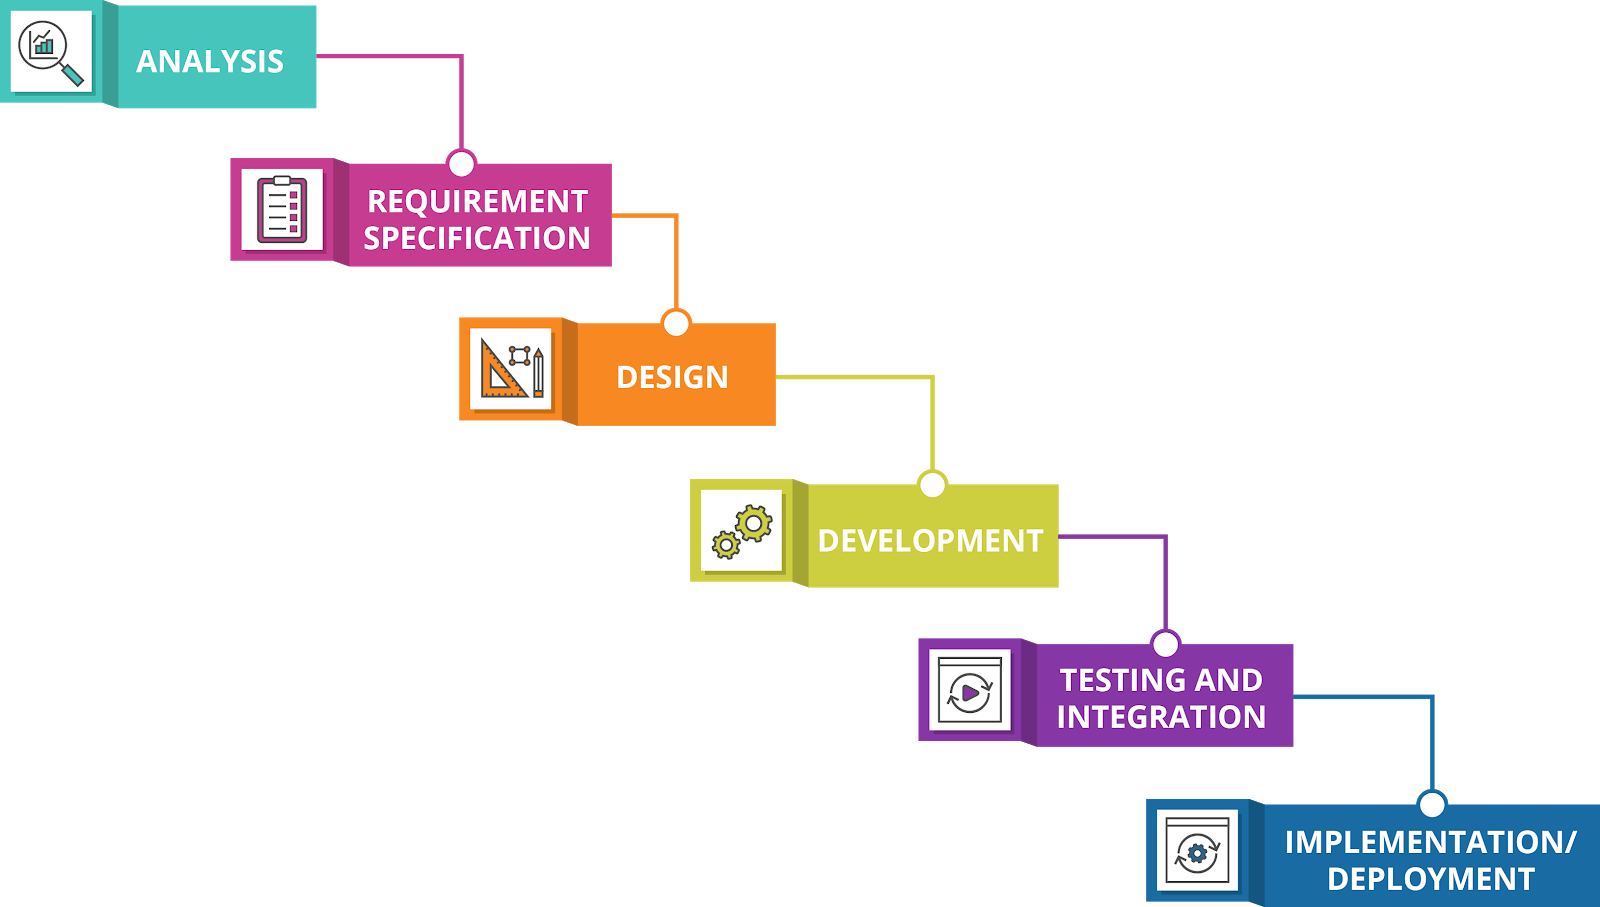
\includegraphics[width=0.8\textwidth]{waterfall}
					\caption{Modello Waterfall}
					\label{fig:waterfall}
				\end{figure}
				
				\paragraph{Waterfall}
				Il processo di sviluppo storicamente più tradizionale e semplice è chiamato \emph{Waterfall}.
				Il nome suggerisce come, rispetto alle fasi del ciclo di vita del software, queste vengano eseguite in "cascata",
				dove la fine di una fase permette di iniziare quella successiva, seguendo ciò che era stato appreso dalla produzione
				manufatturiera applicandolo in ambito dello sviluppo software.
				
				\vspace{5mm}
				La creazione di tale processo ha permesso di superare i limiti del processo \emph{code and fix}, permettendo di pianificare
				in modo più strutturato e dividendo in modo netto le problematiche in base alla fase di appartenenza.
				Altrettante sono però state le problematiche derivanti dalla sua applicazione, tra cui:
				\begin{itemize}
					\item Le fasi di \emph{alpha/beta} testing ripercorrono per natura tutte le fasi del processo, rallentando lo sviluppo;
					\item Ogni fase viene congelata dopo la sua fine, rendendo impossibile la comunicazione tra clienti e sviluppatori dopo la fase iniziale;
					\item La pianificazione viene effettuata solo all'inizio, orientando lo sviluppo ad una data specifica di rilascio; Ogni errore porta a ritardare tale data, che non può però essere stimata di nuovo;
					\item La stima dei costi e delle risorse si rende difficile senza la prima fase di Analisi;
					\item La specifica di requisiti vincola il prodotto da sviluppare, mentre nei casi reali spesso le necessità del cliente cambiano in corso d'opera, specialmente sul lungo termine;
				\end{itemize}
	
				\begin{figure}[h]
					\centering
					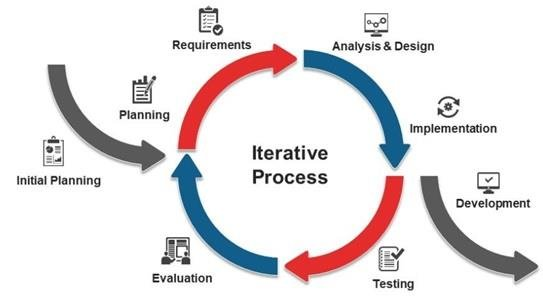
\includegraphics[width=0.6\textwidth]{iterative}
					\caption{Modello Iterativo}
					\label{fig:iterative}
				\end{figure}
	
				\paragraph{Iterativo}
				Una evoluzione del processo \emph{Waterfall} è il modello \emph{Iterativo}, basato sullo stesso ciclo di vita descritto precedentemente, ma con un sostanziale cambiamento che lo rende la base dei modelli odierni, ovvero il riconoscimento che
				lo sviluppo di un software non è composto di una singola iterazione del flusso ma di diverse iterazioni, sempre incrementali.
				
				\vspace{5mm}
				L'idea alla base del modello \emph{Iterativo} consta nel ripetere il ciclo di sviluppo più volte, in porzioni di tempo più ristrette,
				permettendo agli sviluppatori di apprendere dai cicli precedenti e di migliorare i successivi, grazie alla continua
				revisione dei requisiti e del design del software.
				
				\vspace{5mm}
				Il processo parte con una prima iterazione volta a creare un prodotto basilare ma usabile, in modo da raccogliere il feedback
				dell'utente o cliente da utilizzare come input per il ciclo successivo. Per guidare le varie iterazioni, si sfrutta una lista
				di tasks necessari per lo sviluppo del software, che include sia nuove feature sia modifiche al design provenienti da iterazioni
				precedenti, da aggiornare in ogni fase di analisi (per ogni iterazione).
				
				Confrontato con \emph{Waterfall}, il modello \emph{Iterativo} porta diversi vantaggi:
				\begin{itemize}
					\item L'utente viene coinvolto ad ogni iterazione, migliorando il feedback e la qualità del prodotto finale;
					\item Ogni iterazione incrementale produce un \emph{deliverable} che può essere accettato dall'utente, e solo dopo ciò si potrà procedere alla prossima iterazione;
					\item Ogni iterazione permette di rimodulare le risorse necessarie allo sviluppo, così da attuare tecniche di cost-saving;
					\item Il prodotto può essere consegnato fin dalla prima iterazione, seppur in fase embrionale ma funzionante;
					\item Il modello \emph{Iterativo} può essere applicato anche a progetti di piccole dimensioni con successo.
				\end{itemize}
	
		\section{Modelli \emph{Agile}}
	
			\begin{figure}[h]
				\centering
				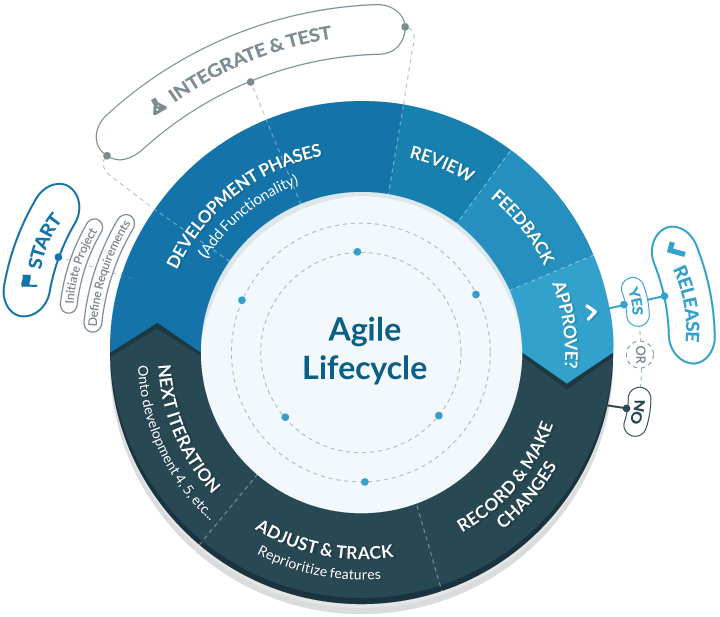
\includegraphics[width=0.8\textwidth]{agile}
				\caption{Modello Agile Generico}
				\label{fig:agile_generic}
			\end{figure}
	
			\subsection{La filosofia \emph{Agile}}
				
				La filosofia \emph{Agile} è emersa a partire dai primi anni 2000, grazie alla pubblicazione del \href{https://agilemanifesto.org/iso/it/principles.html}{\emph{"Manifesto for Agile Software Development"}} nel 2001, nato dall'evoluzione dei metodi classici iterativi ed incrementali.
				
				L'utilizzo di questa filosofia permette di ridurre sensibilmente il rischio di errori dovuti alla male interpretazione dei
				requisiti o il ritardo nelle tempistiche di consegna del prodotto finale, ponendo il focus sulla \textbf{adattabilità} dei processi al cambiamento e sulla \textbf{soddisfazione} del cliente come metrica di successo di un processo di sviluppo.
				Ciò è permesso grazie alla suddivisione dello sviluppo in \textbf{iterazioni} di piccole dimensioni (generalmente 1-3 settimane),
				permettendo un rilascio continuo del software in modo incrementale, e dall'attuazione di alcuni principi tra cui:
				
				\begin{itemize}
					\item \textbf{Individui e interazioni}: nello sviluppo \emph{Agile}, auto-organizzazione e motivazione sono importanti tanto quanto le interazioni tra persone e il pair programming;
					\item \textbf{Software Funzionante}: viene consegnato frequentemente software funzionante in tempi preferibilmente brevi, sotto forma di \emph{Demo};
					\item \textbf{Collaborazione col Cliente}: committenti a sviluppatori devono lavorare insieme quotidianamente per tutta la durata del progetto;
					\item \textbf{Risposta al Cambiamento}: lo sviluppo \emph{Agile} si concentra nel fornire una risposta veloce ai cambiamenti nei requisiti, anche in fasi avanzate dello sviluppo;
					\item \textbf{Gestione delle Priorità}: lo sviluppo inizia solo dopo aver messo in priorità gli obiettivi, spesso utilizzando una tecnica chiamata \emph{MoSCoW} (\emph{Must - Should - Could - Won't Have});
					\item \textbf{Timeboxing}: suddividere il progetto di sviluppo in intervalli temporali ben definiti, spesso di pochi giorni o settimane, entro il quale consegnare alcune features, contenuti in intervalli più lunghi di consegna del prodotto finale o di una parte di esso.
				\end{itemize}
			
				I modelli \emph{Agile} presentano diversi vantaggi che han permesso la loro adozione nella maggior parte degli ambienti di sviluppo software, tra cui:
				\begin{itemize}
					\item I processi sono molto \textbf{realistici} e riflettono il mercato;
					\item Promuovono il lavoro in team e il cross-training;
					\item Le funzionalità vengono sviluppate velocemente e dimostrate al cliente;
					\item Utilizzabili sia con requisiti fissati che in continuo cambiamento;
					\item Pianificazione ridotta al minimo;
					\item Facilità di gestione.
				\end{itemize}
			
				Contemporaneamente portano anche alcuni svantaggi, derivanti dalla flessibilità del processo e quindi dalla non applicabilità in tutti i casi esistenti:
				\begin{itemize}
					\item Difficoltà di gestione di dipendenze complesse;
					\item Rischio aumentato sulla sostenibilità e mantenibilità del processo;
					\item Necessità di un piano di lavoro generale, e di \textbf{figure chiave} per far funzionare il processo;
					\item Forte dipendenza dal feedback del cliente, per colpa di cui il team potrebbe essere direzionato in modo errato.
				\end{itemize}
	
			\subsection{Un modello di successo: SCRUM Framework}
			
				\begin{figure}[h]
					\centering
					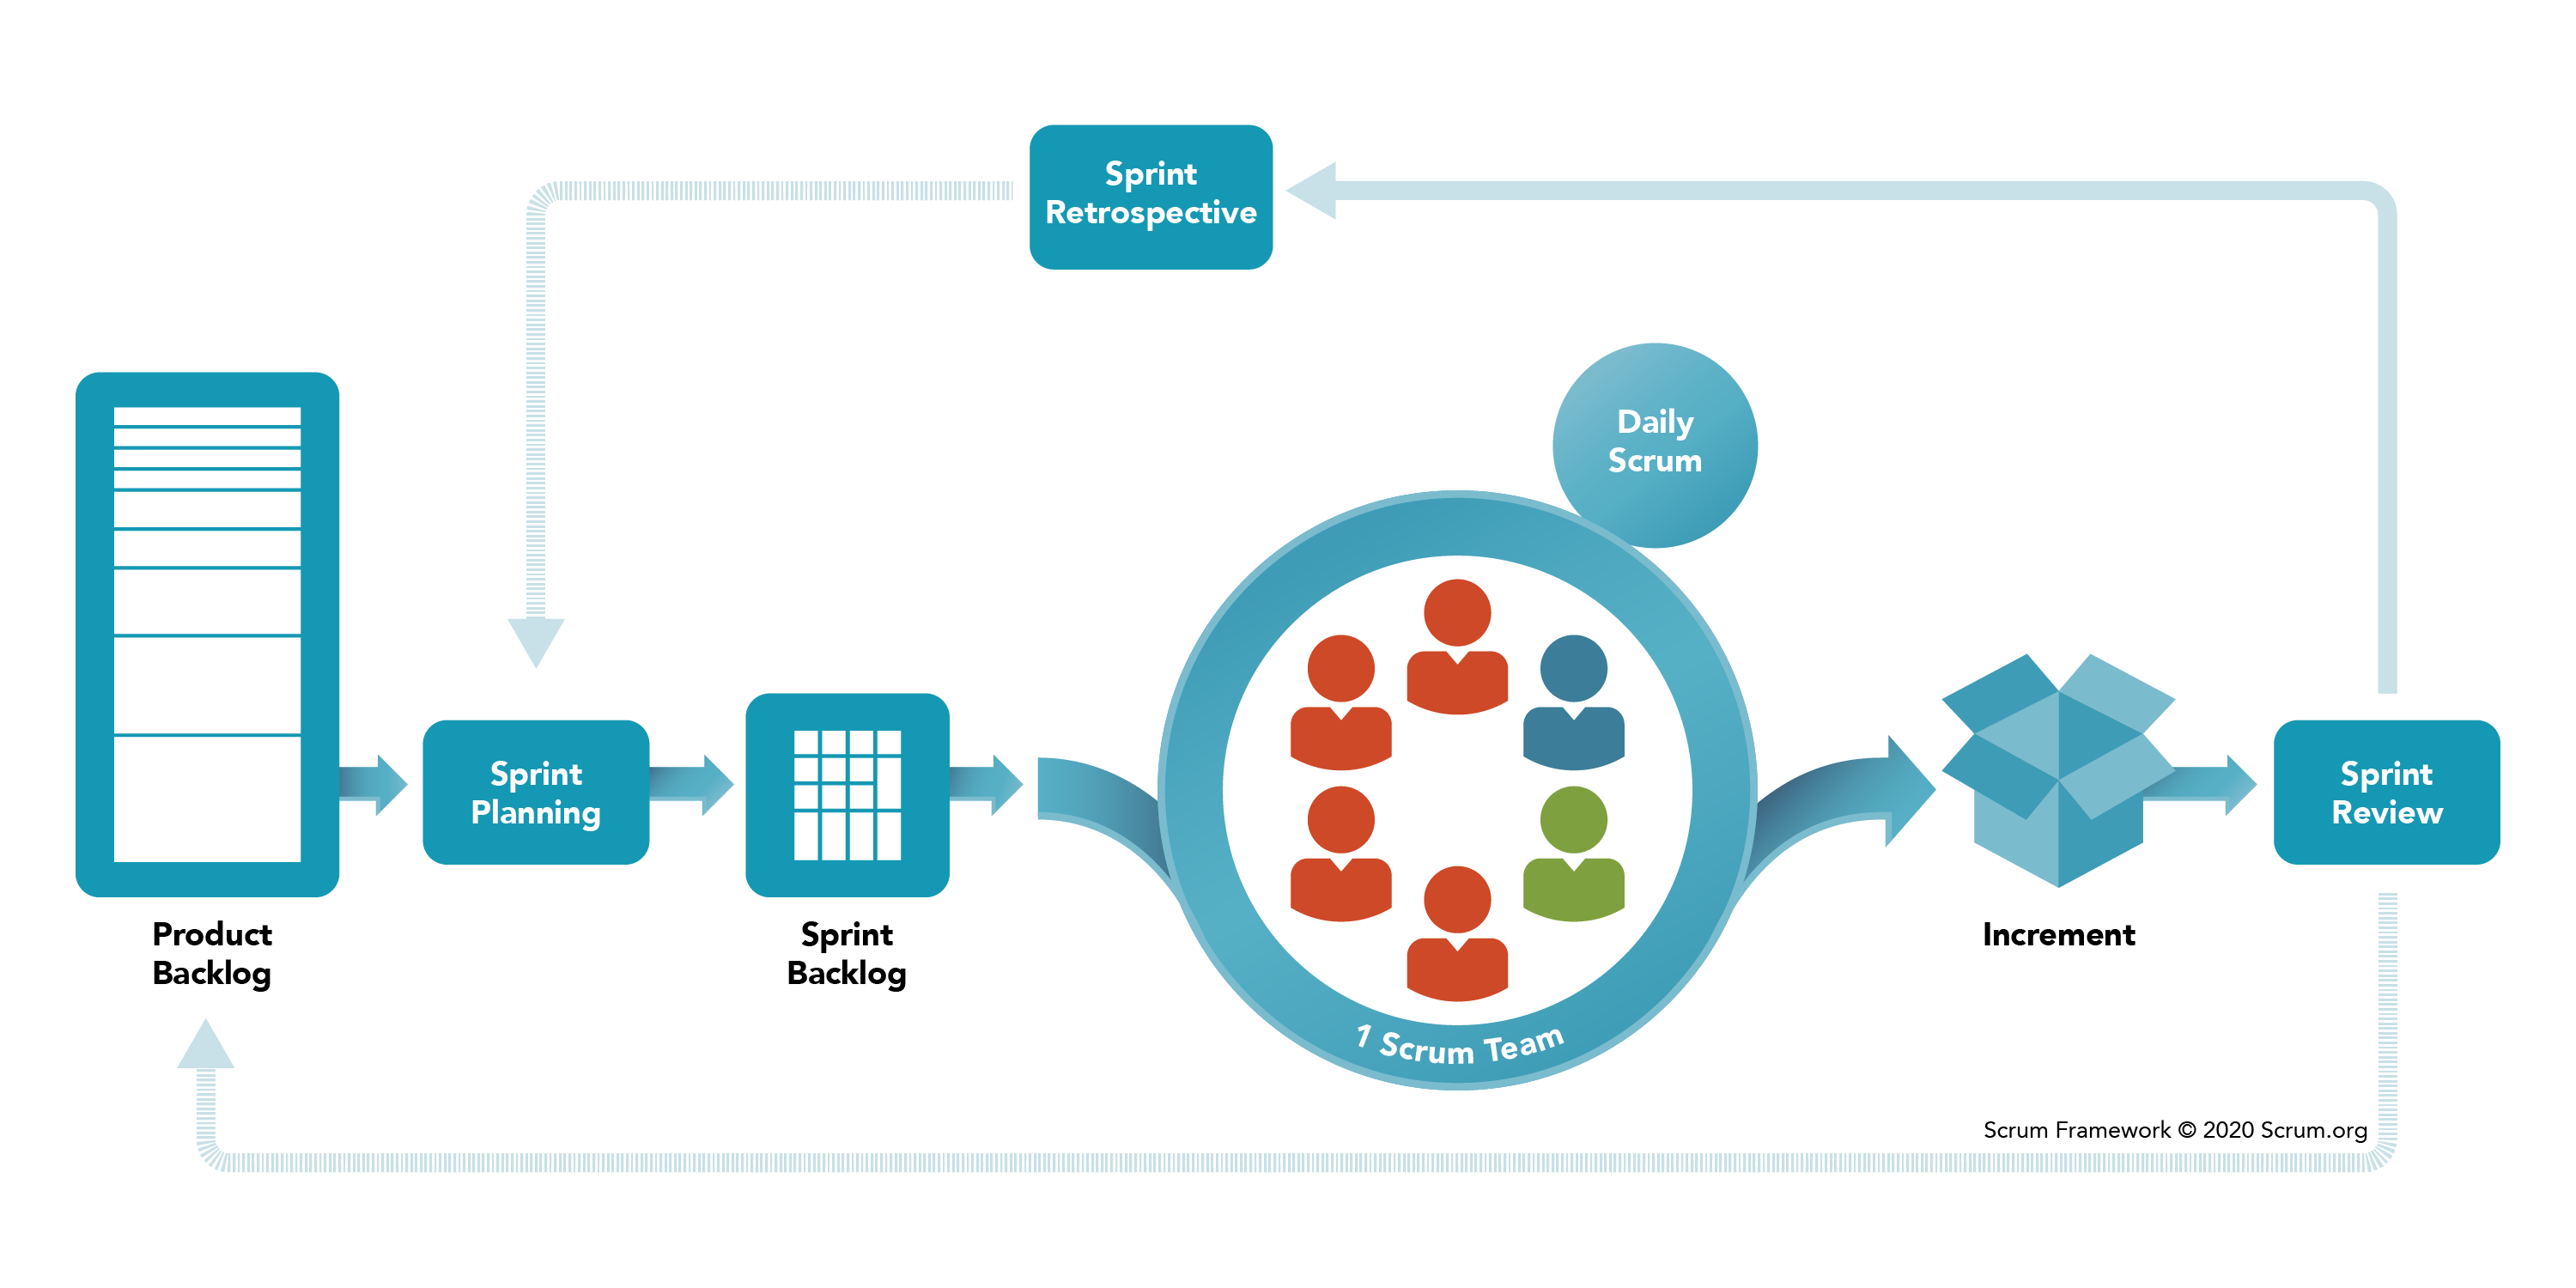
\includegraphics[width=1\textwidth]{scrum}
					\caption{SCRUM Framework}
					\label{fig:scrum}
				\end{figure}
			
				Nel mondo \emph{Agile} sono nati diversi metodi e processi con approcci differenti alla filosofia precedentemente descritta, uno dei quali è \textbf{SCRUM Framework}, il più diffuso ed utilizzato nel mondo dello sviluppo software.
				
				Il termine \textbf{SCRUM} deriva dal gioco del \emph{Rugby}, più precisamente dal pacchetto di mischia, e viene usato
				come metafora del team di sviluppo che deve lavorare insieme in modo che tutti gli attori del progetto \emph{spingano}
				nella stessa direzione, agendo come una unica entità coordinata.
				
				Notiamo come non stiamo definendo un processo, ma bensì un \emph{framework}, e come tale si propone come
				collezione di metodologie che sposano la filosofia \emph{Agile} ma che possono essere implementate al meglio
				delle proprie possibilità, anche con minimi adattamenti.
				
				\emph{SCRUM} si basa sulla teoria dei controlli empirici di analisi strumentale e funzionale di processo, e si basa
				su alcuni pilastri derivanti da tale teoria:
				\begin{enumerate}
					\item \textbf{Trasparenza}: gli aspetti rilevanti del processo devono essere visibili ai responsabili. Questa trasparenza richiede che venga utilizzato un \emph{linguaggio comune} condiviso da tutti, ed una definizione di
					\emph{done} (finito) condivisa tra gli addetti ai lavori e chi deve accettarlo;
					\item \textbf{Ispezione}: l'uso di SCRUM prevede l'ispezione frequente degli \emph{artefatti} prodotti ed
					i progressi realizzati verso gli obiettivi stabiliti, individuando precocemente eventuali deviazioni.
					La frequenza di tali ispezioni deve essere tale da non rallentare il corso dei lavori, e deve essere effettuato
					da ispettori qualificati;
					\item \textbf{Adattamento}: se durante l'ispezione si trovano difformità oltre i limiti accettabili, bisogna
					intervenire sul processo stesso e sul materiale prodotto. L'intervento deve essere portato a termine il più
					velocemente possibile per evitare ulteriori ripercussioni e ridurre al minimo le perdite. Vengono quindi definite
					quattro occasioni per ispezione e adattamento:
					\begin{itemize}
						\item Sprint Planning Meeting;
						\item Daily Scrum;
						\item Sprint Review;
						\item Sprint Retrospective.
					\end{itemize}.
				\end{enumerate}
			
				\paragraph{Il Team SCRUM}
				In un processo dove si utilizza \emph{SCRUM}, viene definito il team di sviluppo come \emph{Team SCRUM}, formato da diverse figure:
				\begin{itemize}
					\item \textbf{Product Owner}: rappresenta gli stakeholders (cliente), ed è responsabile del valore business del team.
					Il PO definisce gli \emph{item} (requisiti di prodotto) in base ai bisogni dei clienti (usando \emph{user stories}),
					assegnando la loro priorità e li inserisce nel \emph{product backlog};
					\item \textbf{Team di Sviluppo}: l'insieme degli sviluppatori responsabili della consegna del prodotto, con incrementi
					potenzialmente rilasciabili alla fine di ogni \textbf{Sprint}. Il team è composto da un numero di persone che varia da 3 a 9, con competenze cross-funzionali e che si auto-organizza;
					\item \textbf{Scrum Master}: responsabile della rimozione di ostacoli che potrebbero limitare la capacità produttiva
					del team e quindi di raggiungere gli obiettivi dello \emph{Sprint}. Sebbene possa sembrare un ruolo manageriale,
					lo Scrum Master è solo il supervisore del processo, detta l'autorità relativa alla applicazione delle norme e presiede
					le riunioni importanti, e funge da protezione al team di sviluppo che può così concentrarsi sullo sviluppo.
				\end{itemize}
			
				\paragraph{Sprint}
				Nello sviluppo \emph{SCRUM}, l'unità base di tempo è chiamato \emph{Sprint}, generalmente di durata di 1-4 settimane.
				Ogni Sprint inizia con una \textbf{riunione di pianificazione}, e si conclude con una \textbf{riunione di revisione} del raggiungimento
				degli obiettivi. Durante lo Sprint non è inoltre permesso cambiare gli obiettivi prefissati all'inizio, che verranno
				quindi tenute in considerazione nell'iterazione successiva.
				
				Al termine di ogni Sprint, il team consegna una versione potenzialmente completa e funzionale del prodotto, contenente
				gli sviluppi conclusi nello Sprint stesso e quelli dei precedenti già conclusi.
				Le funzionalità da sviluppare in uno Sprint provengono dal \emph{product backlog}, come compilato e prioritizzato dal
				\emph{Product Owner}, ed una volta inserite nello \textbf{sprint backlog} non possono essere più aggiunte ne rimosse
				durante il corso dell'iterazione.
				
				\paragraph{Eventi}
				In SCRUM gli eventi vengono sfruttati per \textbf{creare una routine} e ridurre al minimo riunioni al di fuori di quelle definite
				dal framework stesso, tali eventi sono inoltre inclusi nel timeboxing del processo così da integrarsi al meglio con lo sviluppo stesso senza bloccare il team più del dovuto.
				
					\subparagraph{Sprint Planning}
					All'inizio di ogni Sprint, viene effettuato un meeting volto a pianificare le attività dello stesso e gli obiettivi da conseguire entro la sua conclusione, e coinvolge tutto lo Scrum Team. Al suo interno viene definito
					lo \emph{sprint backlog} e si ottiene una stima delle tempistiche e risorse necessarie al suo completamento.
					
					\subparagraph{Daily Scrum}
					Ogni giorno durante lo Sprint, viene effettuata una riunione di comunicazione con tutto il team, in cui ogni componente aggiorna gli altri con la sua situazione di sviluppo. Tale meeting viene effettuato nello stesso
					posto e ora ogni giorno, in un tempo ben definito e ridotto (15 minuti massimo), e viene generalmente effettuato
					in piedi (da qui il nome \emph{daily standup}).
					
					\subparagraph{Sprint Review}
					Alla fine dello Sprint viene effettuato un meeting volto a ispezionare l'incremento e adattare, se necessario,
					il \emph{product backlog}. Durante tale riunione il team di sviluppo e gli \emph{stakeholders} collaborano su
					ciò che è stato prodotto durante lo Sprint, viene individuato ciò che è stato "fatto" e non, si discute dei
					problemi incontrati durante lo sviluppo e il \textbf{Product Owner} discute il \emph{product backlog} fornendo una stima dei tempi di sviluppo futuri.
					
					\subparagraph{Sprint Retrospective}
					Questo meeting fornisce al Team Scrum la possibilità di ispezionare se stesso e creare quindi un piano di miglioramento da attuare nelle prossime iterazioni. Durante tale meeting si analizza l'ultimo Sprint riguardo
					persone, processi e strumenti, così da identificare i punti di miglioramento e cosa invece ha funzionato correttamente. Lo Scrum Master fornisce un ruolo chiave durante la retrospettiva, incoraggiando il team a migliorarsi,
					e aiutando a trovare i punti di discussione.
							
			\subsection{Un modello veloce: eXtreme Programming}
	
		\section{Metodologie di Sviluppo \emph{Agile}: DevOps}
	
			\subsection{Un metodo ed un'etica}
			
			\subsection{Obiettivi delle pratiche DevOps}
			
			\subsection{Processo di Riferimento}
	
				\subsubsection{Continuous Integration}
				
				\subsubsection{Continuous Delivery}
				
				\subsubsection{Continuous Deployment}
	
		\section{Il ROI del DevOps}
	
	\chapter{Sviluppo ed Automazione su Cloud}
	
	\section{Perchè il Cloud?}
	
	\section{\emph{Infrastructure-as-a-Code}}
	
	\section{\emph{Configuration-as-a-Code}}
	
	\section{Containers ed ambienti controllati}
	
	\chapter{Analisi del Processo di Sviluppo}
	
	\section{Struttura del Progetto}
	
	\section{Il processo di sviluppo}
	
	\section{Requisiti e KPI}
	
	\section{Il processo DevOps}
	
	\subsection{Architettura High-Level e Fasi}
	
	\subsection{Gestione del Codice}
	
	\subsection{Pull Requests e Code Review}
	
	\subsection{Continuous Integration}
	
	\subsubsection{Test Automation}
	
	\subsubsection{Code Analysis}
	
	\subsection{Continuous Delivery}
	
	\subsubsection{Build Automation}
	
	\subsubsection{Artifacts Delivery}
	
	\subsection{Deployment}
	
	\section{Tecnologie e Strumenti}
	
	\subsection{SCM: Git}
	
	\subsection{Build System: Bazel}
	
	\subsection{Cloud Provider: AWS}
	
	\subsection{PR Management: Phabricator ed Arcanist}
	
	\subsection{CI/CD: Jenkins}
	
	\subsection{Code Analysis: SonarQube}
	
	\chapter{Tecnologie di Background}
	
	\section{Cloud Provider: \emph{AWS}}
	
	\section{Infrastructure-as-a-Code: \emph{Terraform}}
	
	\section{Configuration-as-a-Code: \emph{Ansible}}
	
	\section{Container Engine: \emph{Docker}}
	
	\chapter{Architettura Cloud}
	
	\section{Diagramma Architetturale}
	
	\section{Configurazione di Phabricator}
	
	\section{Configurazione di Jenkins}
	
	\subsection{Agent su AWS EC2}
	
	\subsection{Agent macOS On-Premise}
	
	\section{Configurazione di SonarQube}
	
	\section{Creazione ambiente di build con Docker}
	
	\chapter{La Pipeline di CI}
	
	\section{Tecnologie e Strumenti}
	
	\subsection{Phabricator ed Arcanist: un flusso controllato}
	
	\subsection{Jenkins: il motore del processo}
	
	\subsection{Docker: ambiente di testing unificato}
	
	\subsection{SonarQube: controllo qualità}
	
	\section{Le fasi della Pipeline}
	
	\section{Analisi del Codice}
	
	\subsection{Quality Gates}
	
	\subsection{Code Coverage}
	
	\subsection{Risposta a cambiamenti nella qualità}
	
	\section{Risultati di Testing e QA}
	
	\chapter{La Pipeline di CD}
	
	\section{Tecnologie e Strumenti}
	
	\subsection{Jenkins: il motore del processo}
	
	\subsection{Docker: ambiente di build unificato}
	
	\section{Le fasi della Pipeline}
	
	\section{Analisi delle Vulnerabilità}
	
	\section{Risultati}
	
	\chapter{Conclusioni}
	
	\section{Obiettivi Raggiunti}
	
	\section{Risultati su Requisiti e KPI}
	
	\section{Evoluzioni Future}
	
	\section{Considerazioni Personali}
	
\end{document}